\chapter{基于预训练模型的参考服务方法}

\section{参考服务问题描述}
如今随着互联网的浪潮,许多传统行业也加快了信息化的脚步,也在朝着服务化的方
向转型,许多互联网企业关注的重点也从线上延伸到线下,如何通过互联网的方式,整合
线下资源,提供更优质和便捷的服务成了新的创业方向,也促进了线下的产业拥抱互联网,
形成互联网+。医疗行业作为关系国计民生的重要行业,为解决当前老百姓看病难,看病
贵等问题,也迫切需要结合新兴的信息技术提高医疗服务水平。目前很多医院的信息化水
平还比较低,使用着老旧的HIS 院内系统,而且各家医院的HIS 系统都是由不同的公司独
立开发,彼此之间差异较大,互相连通的难度也比较大。当下也有许多互联网医疗公司和
平台,致力于通过互联网的手段,来整合线下的医疗资源,并希望最大化利用好这些医疗
资源,为医生和患者提供更简洁方便的就医和就诊体验,比如春雨医生、好大夫在线,丁
香医生等等。

目前互联网医疗类的创业公司正处于百花齐放的高速发展阶段,各家业务的侧重点也
不尽相同,然而不论这些公司的业务差异,它们大多都有对接线下实体医院信息系统的诉
求,因为它们往往都需要线下这些实体医院作为支撑才能开展它们的业务。目前这些公司
都需要一家一家的去和线下的医院谈合作,达成合作之后还要进行院内系统的对接工作,
由于线下医院的数量众多,而且各家院内系统没有统一的规范,都不尽相同,所以这意味
着巨大的工作量,劳财费力,经常是事倍功半。反过来,对于医院来说,它们经常面临很
多家类似的互联网医疗企业的合作请求,处理起来也是非常麻烦,而且医院更希望形成医
院之间的服务网络,这对于病人的转诊,医生的跨院会诊等当前这些需要跨院交流的活动
会提供很大的流程简化和便捷,而且形成医院之间的服务网络之后,能够更加充分的整合
和调度各家医院之间的医疗资源,能够达到最大化利用这些医疗资源为社会提供更好的医
疗服务。

类似的情况不仅仅是在医疗这个领域出现,几乎每个领域在面临信息化,拥抱互联网
+ 的过程,甚至互联网企业在构建自己服务的同时,都会面临这样的问题。从形成公司内
部的服务网络,到公司或组织之间的服务网络,再到某个行业的服务网络,最终发展成全
行业互相连通的服务网络,这个趋势不可逆转。

\begin{figure}[htbp]
    \centering
    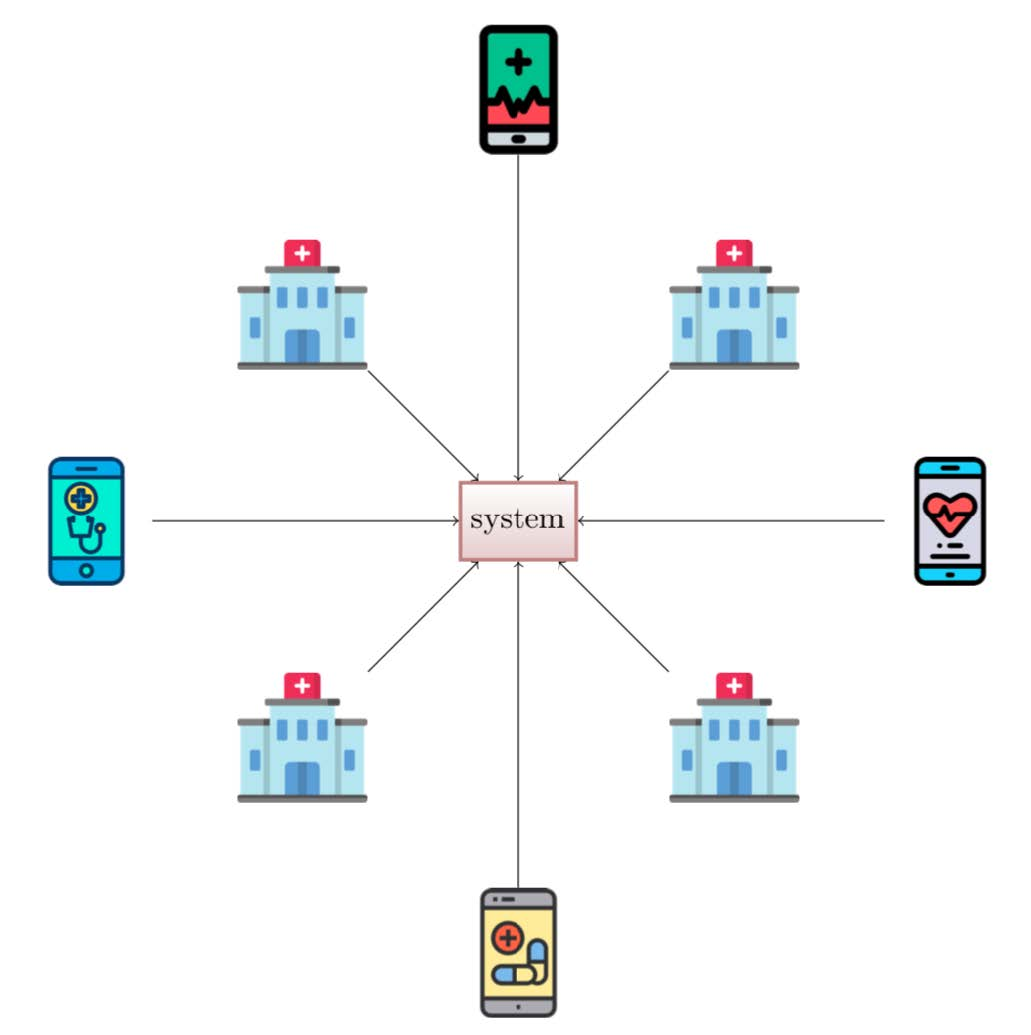
\includegraphics[scale=0.5]{./images/serverAdvise.jpg}
    \caption{互联网医院服务接入示意图}
    \label{fig:serverAdvise}
  \end{figure}

从互联网医疗的案例中我们可以看出,随着现代化服务水平的不断提升,形成一个行
业内,甚至跨行业的服务网络是必然趋势。构建一个完整、和谐、不断进化的服务生态系
统是我们的追求。当前的服务生态系统还远远不够完善,对于服务消费者和服务提供者来
说都存在着诸多不便。我们的整体解决方案是提出一个服务运营商的概念,上联服务消费者,下联服务提供
者,负责建设、完善和运营整个服务生态。具体来说,对于服务提供者,他们将自己的服务开放注册到我们的平台,我们提供了
自动化工具,我们负责统一化、语义标注等工作,方便统一管理和使用,对于服务消费者,
我们提供自定义服务的功能,简化服务使用流程、颠覆服务使用体验、避免服务升级、服
务选择等问题。对于互联网医疗的案例,通过我们的解决方案,医院将它们的开放API 注册到我们的
系统后,任何互联网医疗企业,只需要接入我们的平台,便可直接和海量的医院资源连通,
避免了海量的重复工作和资源浪费,节约了企业的精力,能让它们更好的聚焦于公司的业
务。

在这其中,服务接入时实体服务对系统内部标准服务的映射显然是最为关键的一环。

\section{预处理与算法描述}

\subsection{跨界服务网络平台内标准服务的构建}

接上一小节所述,要想做到上联服务消费者,下联服务提供者,对每一类具体的服务,在跨界服务平台内部就必须要有统一的标准来衡量。
因此,我们提出了标准服务的概念。同时,我们在服务研究领域展开调研,遗憾的是,没有发现相关的公开数据集,相关的资料更是少之又少。
针对标准服务的现状,我们构建了自己的标准服务集,标准服务的属性值对应到nre问题即为一个个实体。

本文实体服务的主要来源有主流的web API开放平台,包括京东万象数据服务商城,聚合数据,ProgramWeb等。对于医疗这一特定领域的服务,实验室课题组
与浙江医院,邵逸夫医院等多家有合作,借助实验室已有项目医联体获得了大量的医疗系统相关的服务api。本文通过调研选取了用户量较多的六大领域(医疗健康,生活服务,
交通地理,金融科技,饮食文娱,电子商务),从这六大用户比较热门的领域中构建标准服务。

\begin{table}[htb]
    \centering
    \caption{标准服务数据集}
    \label{tab:RelatedResearchAbroad}
      \begin{tabular}{p{4cm}|p{4cm}|p{6cm}}
        \toprule
        % & \multicolumn{1}{m{60mm}}{\heiti\centering 相关研究成果}
        \multicolumn{1}{l|}{\heiti 实体类别} & \multicolumn{1}{l|}{\heiti 实体数} & \multicolumn{1}{l}{\heiti 占比(\%)}\\
        \midrule
        % IBM & 服务科学、服务工程;\\
        医疗健康 & 126 & 31.19\\ \hline
        生活服务 & 109 & 26.98\\ \hline
        交通地理 & 63 & 15.59\\ \hline
        金融科技 & 26 & 6.43\\ \hline
        饮食文娱 & 58 & 14.28\\ \hline
        电子商务 & 24 & 5.53\\ \hline
        总计 & 406 & 100.00\\ \hline
        % \rowcolor[gray]{.9} colortbl & 表格上色。自己看着爽而已,打印出来都是黑白的。 \\
        % threeparttable & 用来给表格添加脚注啥的很方便。 \\
        % array & 忘了用来做什么了,但似乎很重要。 \\
        \bottomrule
      \end{tabular}
  \end{table}

  \subsection{结构化表示}
  想要把实体服务的参数信息输入神经网络中,数字化表示是第一步,词嵌入(Word embedding)是文本词汇最流行的表示形式之一,
  它是特定单词的向量表示,它能够捕获文档中单词的上下文,语义和句法相似性,与其他单词的关系等。

  标签的结构化表示

  \subsection{结构化表示}




\section{基于深度学习的参考服务方法}
本小节主要介绍跨界服务中服务映射(参考服务)问题的一种深度学习方法



